\documentclass[12pt]{article}
\usepackage{geometry}
\usepackage{url}
\usepackage{graphicx}
\usepackage{float}
\usepackage{pdflscape}
\usepackage{amsmath}
\title{\Huge Neural Networks \\
[6mm]
Assignment 3\\}
\author{Ravikiran Bhat\\
Rubanraj Ravichandran\\
Ramesh Kumar}

\begin{document}
\maketitle
\newpage
\section{Exercise 2.1}
The equation 2.3 gives the weight adjustment $\Delta w_{kj}$ applied to synaptic weight $w_{kj}(n)$ according to the delata rule: \\
$$\Delta w_{kj} = \eta e_{k}(n) x_{j}(n)$$  
The equation 2.9 gives the weight adjustment $\Delta w_{kj}$ as: $$\Delta w_{kj} = \eta y_{k}(n) x_{j}(n)$$  
The main distinguishing feature between these two rules is that in case of the delta rule, the adjustment to synaptic weight of a neuron is proportional to the product of the error signal and input signal of the synapse, whereas the Hebb's rule gives the synaptic weight $w_{kj}$ for neuron k as a function of presynaptic signal (i.e, the input signal) and postsynaptic signal (i.e, the output signal).
\newpage   
\section{Exercise 2.10:}
\begin{figure}[h]
	\begin{center}
		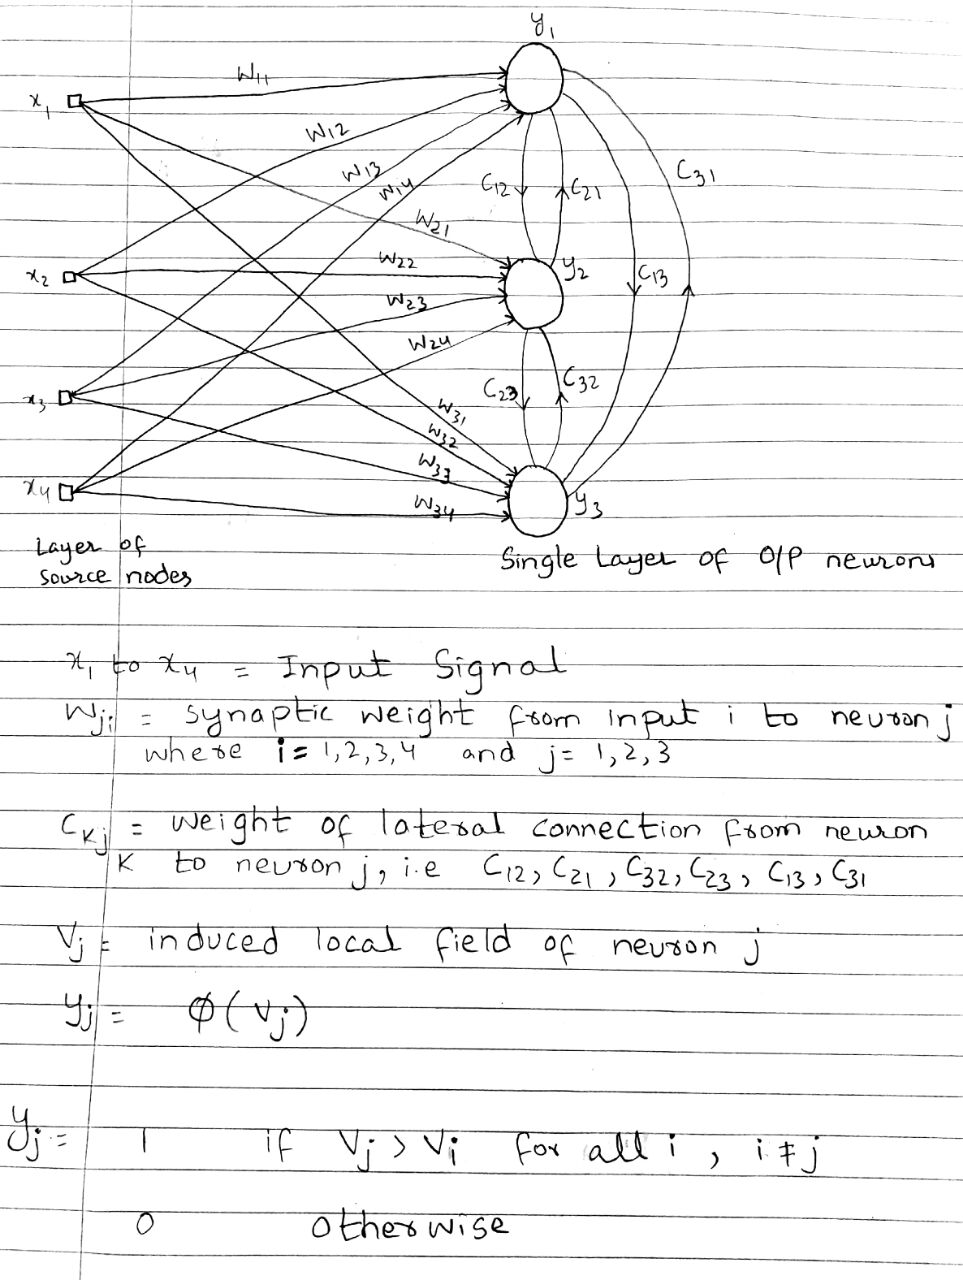
\includegraphics[width = 15cm, height = 11cm]{2_10.jpg}
	\end{center}
\end{figure}
Weight adjustment can be written as:
\begin{figure}[h]

			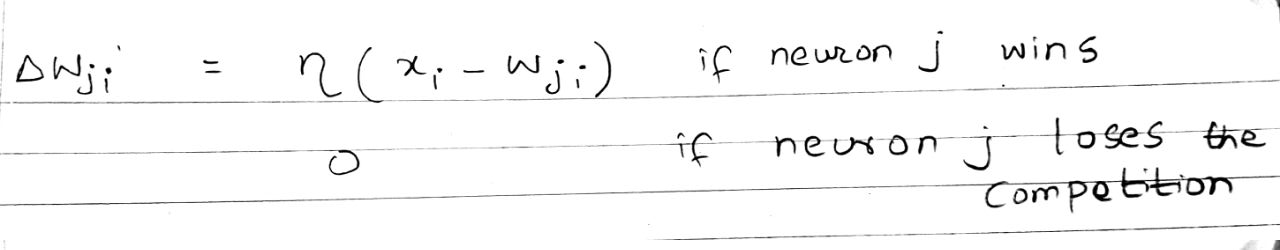
\includegraphics[scale = 0.30]{2_10a.jpg}

\end{figure}

The local field generated for a neuron should be larger than other neurons local field.
Local field of neuron 'k' is nothing but, sum of the vector products of input 'j' and synapse weight 'k'.  
Let say, there are 3 output neurons in the network and the local field of neuron 2 is greater than neuron 1 and 3.
In this case the neuron 2 is the winner and we update only the synapse weights which is connected with neuron 2.

$$y_j = \phi(\sum_{i=1}^{4} w_{ji}x_i  + \sum_{k=1, k \neq j}^{3} c_{kj}y_k)$$, where $k_1, k_2$ are numbers from 1 to 3 those are not equal j.

\end{document}